% ****************************************************************************************************
\chapter{Proof of Concept -- The Example of SAP HANA Cloud}\label{ch:poc}
% ****************************************************************************************************

In order to evaluate and show the applicability of the previously developed \ac{DSR} artifacts, i.e. the classification scheme (cf. Chapter \ref{ch:sota}), \ac{CLD} (cf. Chapter \ref{ch:cld}), and \ac{SFD} (cf. Chapter \ref{ch:sfd}), now a \acf{PoC} study using the example of the SAP HANA Cloud platform is presented. This approach is in conformity with the \ac{DSR} design cycle of \citet[pp. 88,90-91]{Hevner2007} and the \ac{DSR} activity evaluation according to \citet[p. 56]{Peffers2007}, whereby the artifacts have been evaluated against the real world by their reapplication in the context of \ac{PaaS} business models.

% ****************************************************************************************************
\section{Classification}\label{ch:poc:cs}
% ****************************************************************************************************

The business model of the SAP HANA Cloud platform is explained and illustrated in detail in Subsection \ref{ch:sota:sap}, using the business model conceptualization proposed by \citet{Johnson2008}. In order to classify \ac{PaaS} business models, a corresponding classification scheme has been developed. The way the SAP HANA Cloud platform addresses each of the classification criteria identified above is briefly discussed below and illustrated in Figure \ref{fig:cs:sap} by means of a morphological box, where the characteristics addressed are highlighted.

In the analysis of this platform, four diverse stakeholder groups which are directly targeted were identified: application customers, development partners, platform customers, and individual developers. Using the terminology of the classification scheme, the SAP HANA Cloud platform addresses all five identified customer segments: \ac{IT} startup, \ac{SI}, \ac{ISV}, platform customers, as well as application customers. However, these customer segments are served differently, as illustrated further below. SAP HANA Cloud aims to support the development, deployment, and management of standalone as well as integrated cloud solutions. However, the focus of this platform is to provide extensive features for integration and is thus classified as a \ac{PaaS} platform with the core value proposition 'integration'. The SAP HANA Cloud platform is neither an open source platform nor a highly regulated platform, hence a partly limited governance model is pursued, meaning platform users of all kinds have an extensive freedom of choice, although certain areas are regulated directly by the platform provider. Even though the SAP HANA Cloud platform offers several technical capabilities, for instance the SAP Hana Cloud Eclipse plugin and corresponding \ac{SDK}, they are considered limited and thus regarding the criterion technical scope, the characteristic limited technical capabilities is selected. In particular, the comparison with other \ac{PaaS} platforms and their technical capabilities supports this classification. Based on the SAP HANA Cloud platform case study, three revenue streams, used by the platform provider, can be identified. First, platform customers are charged subscription-based fees ranging from $370$ to $16.000$ \ac{EUR} monthly. Second, SAP retains a revenue share of $15\%$ for platform modules developed by complementors, both \acp{ISV} and \ac{IT}, and distributed through the SAP Store. Third, some additional services are offered at a fee, including annual development partner fees of $1.990$ \ac{EUR} and application certification fees ranging from $495$ to $990$ \ac{EUR}.

\begin{figure}[tb]
	\centering
	% ****************************************************************************************************
% Classification Scheme SAP
% ****************************************************************************************************

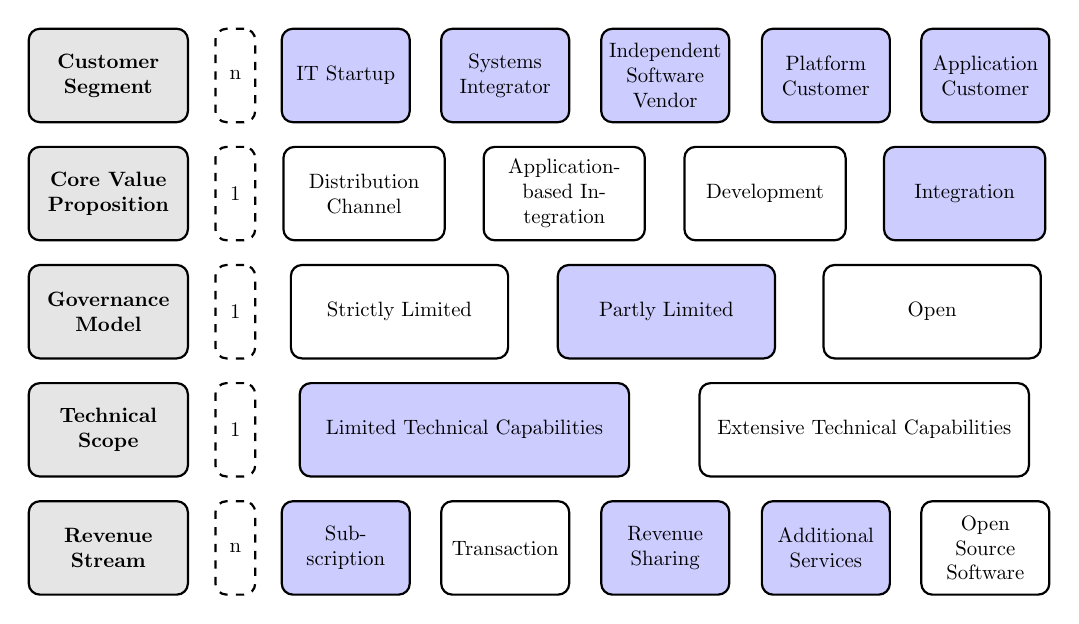
\begin{tikzpicture}[scale=0.75, every node/.style={scale=0.75}]

\node[font={\bfseries},draw,text width=7em,text centered,rectangle,rounded corners,minimum height=4.5em,thick,fill=gray!20] (1) at (-1,8) {Customer Segment};
\node[font={\bfseries},draw,text width=7em,text centered,rectangle,rounded corners,minimum height=4.5em,thick,fill=gray!20] (1) at (-1,6) {Core Value Proposition};
\node[font={\bfseries},draw,text width=7em,text centered,rectangle,rounded corners,minimum height=4.5em,thick,fill=gray!20] (1) at (-1,4) {Governance Model};
\node[font={\bfseries},draw,text width=7em,text centered,rectangle,rounded corners,minimum height=4.5em,thick,fill=gray!20] (1) at (-1,2) {Technical Scope};
\node[font={\bfseries},draw,text width=7em,text centered,rectangle,rounded corners,minimum height=4.5em,thick,fill=gray!20] (1) at (-1,0) {Revenue Stream};

\node[draw,text width=1.25em,text centered,rectangle,rounded corners,minimum height=4.5em,thick,dashed] (1) at (1.15,8) {n};
\node[draw,text width=1.25em,text centered,rectangle,rounded corners,minimum height=4.5em,thick,dashed] (1) at (1.15,6) {1};
\node[draw,text width=1.25em,text centered,rectangle,rounded corners,minimum height=4.5em,thick,dashed] (1) at (1.15,4) {1};
\node[draw,text width=1.25em,text centered,rectangle,rounded corners,minimum height=4.5em,thick,dashed] (1) at (1.15,2) {1};
\node[draw,text width=1.25em,text centered,rectangle,rounded corners,minimum height=4.5em,thick,dashed] (1) at (1.15,0) {n};

\node[draw,text width=5.5em,text centered,rectangle,rounded corners,minimum height=4.5em,thick,fill=blue!20] (1) at (3.02,8) {IT Startup};
\node[draw,text width=5.5em,text centered,rectangle,rounded corners,minimum height=4.5em,thick,fill=blue!20] (1) at (5.72,8) {Systems Integrator};
\node[draw,text width=5.5em,text centered,rectangle,rounded corners,minimum height=4.5em,thick,fill=blue!20] (1) at (8.43,8) {Independent Software Vendor};
\node[draw,text width=5.5em,text centered,rectangle,rounded corners,minimum height=4.5em,thick,fill=blue!20] (1) at (11.15,8) {Platform Customer};
\node[draw,text width=5.5em,text centered,rectangle,rounded corners,minimum height=4.5em,thick,fill=blue!20] (1) at (13.85,8) {Application Customer};

\node[draw,text width=7.1em,text centered,rectangle,rounded corners,minimum height=4.5em,thick] (1) at (3.33,6) {Distribution Channel};
\node[draw,text width=7.1em,text centered,rectangle,rounded corners,minimum height=4.5em,thick] (1) at (6.72,6) {Application-based Integration};
\node[draw,text width=7.1em,text centered,rectangle,rounded corners,minimum height=4.5em,thick] (1) at (10.12,6) {Development};
\node[draw,text width=7.1em,text centered,rectangle,rounded corners,minimum height=4.5em,thick,fill=blue!20] (1) at (13.5,6) {Integration};

\node[draw,text width=9.8em,text centered,rectangle,rounded corners,minimum height=4.5em,thick] (1) at (3.93,4) {Strictly Limited};
\node[draw,text width=9.8em,text centered,rectangle,rounded corners,minimum height=4.5em,thick,fill=blue!20] (1) at (8.45,4) {Partly Limited};
\node[draw,text width=9.8em,text centered,rectangle,rounded corners,minimum height=4.5em,thick] (1) at (12.95,4) {Open};

\node[draw,text width=15.2em,text centered,rectangle,rounded corners,minimum height=4.5em,thick,fill=blue!20] (1) at (5.03,2) {Limited Technical Capabilities};
\node[draw,text width=15.2em,text centered,rectangle,rounded corners,minimum height=4.5em,thick] (1) at (11.8,2) {Extensive Technical Capabilities};

\node[draw,text width=5.5em,text centered,rectangle,rounded corners,minimum height=4.5em,thick,fill=blue!20] (1) at (3.02,0) {Sub-scription};
\node[draw,text width=5.5em,text centered,rectangle,rounded corners,minimum height=4.5em,thick] (1) at (5.72,0) {Transaction};
\node[draw,text width=5.5em,text centered,rectangle,rounded corners,minimum height=4.5em,thick,fill=blue!20] (1) at (8.43,0) {Revenue Sharing};
\node[draw,text width=5.5em,text centered,rectangle,rounded corners,minimum height=4.5em,thick,fill=blue!20] (1) at (11.15,0) {Additional Services};
\node[draw,text width=5.5em,text centered,rectangle,rounded corners,minimum height=4.5em,thick] (1) at (13.85,0) {Open Source Software};

\end{tikzpicture}
	\caption{Proof of Concept -- Classification}
	\label{fig:cs:sap}
\end{figure}

As set out above, the classification scheme developed in this thesis can easily be used for an initial assessment and classification of \ac{PaaS} business models and their characteristics. Hence the classification scheme is shown to be as user friendly as possible, which is a key classification guideline according to \citet[p. 41]{Fettke2003}, while still ensuring that the classification criteria as well as their characteristics are comprehensible and sufficient.

% ****************************************************************************************************
\section{Qualitative Findings}\label{ch:poc:qf}
% ****************************************************************************************************

Based on the previously developed \acp{CLD} (cf. Figures \ref{fig:cld_cs} - \ref{fig:cld_bp}) \ac{PaaS} business models and their inherent dynamics can be investigated, ultimately leading to a better understanding of the effects of these dynamics.

As illustrated in Figure \ref{fig:cld_cs}, six basic factors influencing the \ac{CVP} for all customer segments have been discussed. First, the core value proposition of the SAP HANA Cloud platform which has a direct impact on the \acp{CVP} is focused on integration, as mentioned above. This focus seems appropriate for all five customer segments: complementors, i.e. \acp{ISV} and \ac{IT} startups, developing integration-based platform modules, platform customers developing internal integration solutions, application customers using platform modules for integration purposes, and \acp{SI} providing corresponding consultancy services. Second, the partly limited governance model might also influence the \acp{CVP} for \acp{ISV}, \ac{IT} startups, and platform customers positively, although this might not have much influence on \acp{SI} and application customers. Third, the somewhat limited technical scope (limited technical capabilities) will, in the best case, fail to strengthen the \acp{CVP} especially for \acp{ISV}, \ac{IT} startups, and platform customers. However, in the worst case this limited technical scope will have the opposite effect and negatively influence these \acp{CVP}. Fourth, although some additional services are offered and thus positively influence the \acp{CVP}, particularly for \acp{ISV} and \ac{IT} startups, a broader range of additional services tailored to all targeted customer segments would increase this impact permanently. Fifth, as discussed in Section \ref {ch:cld:cs} and in line with \citet[p. 200]{Evans2003} platform improvements lead to improved \acp{CVP} and also to enhanced technical capabilities as well as a wider range of additional services. Due to the fact that the precise quantities of the variables revenue and investments, which result in platform improvements, are unknown, the actual impact of the self-reinforcing feedback loops R\_2, R\_3, and R\_4 associated with platform improvements (cf. Figure \ref{fig:cld_cs}) is indeterminate. Sixth, the overall market penetration of the SAP HANA Cloud platform is currently small, and its influence on the \acp{CVP} is scarcely perceptible. This impact might change with an increase in the customer base, leading to an increased overall market penetration as indicated by the self-reinforcing feedback loop R\_5 in Figure \ref{fig:cld_cs}.

Using the generic \ac{PaaS} customer segment \ac{CLD}, \ac{PaaS} business models can be analyzed with regard to the adoption dynamics and initial conclusions can be drawn. In case of the SAP HANA Cloud platform, the most significant observation so far concerns the technical scope. Considered individually, and even more in comparison with other \ac{PaaS} platforms offering the same core value proposition of integration, the technical capabilities currently offered are not sufficient. Hence, enlarging the technical scope might lead to substantial \acp{CVP} enhancements.

The inherent and crucial cross-sided network effects between the five \ac{PaaS} customer segments were discussed in Section \ref{ch:cld:csi} and illustrated by means of a \ac{CLD} (cf. Figure \ref{fig:cld_csi}). Since the SAP HANA Cloud platform addresses all five customer segments, this \ac{CLD} cannot be simplified. Nevertheless, valuable insights can be gained.

Platform modules have been shown to influence, both directly and indirectly, all customer segments. These platform complements are developed and provided by complementors, i.e. \acp{ISV} and \ac{IT} startups, and are valuable mainly for platform and application customers, but also for \acp{SI}. However, at present only a few ready-to-use applications built upon the SAP HANA Cloud platform are offered, which might be used by application customers. Hence, the self-reinforcing feedback loops R\_8 and R\_9 (cf. Figure \ref{fig:cld_csi}) will only have weak impacts. Since only a few applications (platform modules) are available, the \ac{CVP} for application customers will remain weak and consequently the application customer population will not increase considerably. This implies that due to the low number of application customers, the \acp{CVP} for \acp{ISV} and \ac{IT} startups are not significantly improved, and thus the number of platform modules stays constant. Furthermore, in order to sell platform modules built upon the SAP HANA Cloud platform via the SAP Store, the so called development partners, i.e. \acp{ISV} and \ac{IT} startups, are charged for the very fact of being such a development partner ($1.990$ \ac{EUR} yearly), and in addition these applications need to go through a certification process ($990$ \ac{EUR} initially, then $495$ \ac{EUR} per year). All these facts and circumstances taken together lead to the unpleasant, but not unusual, situation in which platform providers in their early stages face the so-called chicken-and-egg launch problem. Since this problem is not unfamiliar, several approaches to overcoming it have been developed. For instance, a typical approach to solving this problem is subsidizing one or more customer segments through incentives, as discussed by \citet[pp. 1,5]{Eisenmann2006} and \citet[pp. 195-196]{Evans2003}. The customer segment 'platform customers', on the other hand, is also influenced by platform modules, although less strongly so, because they utilize platform modules in addition to the actual platform itself, i.e. different from the customer segment application customers. Consequently, the feedback loops R\_10 and R\_11 (cf. Figure \ref{fig:cld_csi}) connecting the variables platform customers and platform modules also remain rather weak due to the limited number of platform modules. Finally, since the variables platform customers and application customers as well as platform modules are relatively low, the \ac{CVP} for \acp{SI} is not influenced positively by these factors. As a result, the two self-reinforcing feedback loops R\_6 and R\_7 (cf. Figure \ref{fig:cld_csi}) are almost irrelevant.

The application of the \ac{CLD} artifact developed above (cf. Figure \ref{fig:cld_bp}) to the real-world scenario of the SAP HANA Cloud platform clearly reveals two areas, where SAP might adjust its business model. First, as mentioned above the technical capabilities currently offered are not sufficient and prevent the platform from establishing itself firmly. Extending the technical scope might increase the \acp{CVP} for \acp{ISV}, \ac{IT} startups, and platform customers particularly. Second, so far the SAP HANA Cloud platform does not create significant cross-sided network effects, which have been identified to be essential in the platform adoption process. Instead of experiencing a flourishing platform and its network effects, the common chicken-and-egg launch problem has arisen. SAP might target these cross-sided network effects and try to create and capture more of them in order to overcome this obstacle, for instance by subsidizing quality and/ or price-sensitive customers.

% ****************************************************************************************************
\section{Simulation Results}\label{ch:poc:sr}
% ****************************************************************************************************

\begin{table}[t]
	\centering
	\begin{tabular}{ll}
		\toprule 
		\footnotesize \textbf{Parameter} & \footnotesize \textbf{Value} \\ \midrule
		\footnotesize Initial Time & $0$ \\
		\footnotesize Final Time & $60$ \\
		\footnotesize Time Step & $0.25$ \\
		\footnotesize Time Unit & \footnotesize Month \\ \midrule
		\footnotesize Integration Type & \footnotesize RK4 Auto\footnotemark \\ \bottomrule
	\end{tabular}
	\caption{Proof of Concept -- Simulation Settings}
	\label{tab:tb}
\end{table}

	\footnotetext{RK4 Auto denotes a fourth order Runge-Kutta integration combined with an automatic adjustment of the step size in order to ensure accuracy.}

In Chapter \ref{ch:sfd} the theoretical foundations and the corresponding mathematical formulas of the \ac{SFD} and platform adoption simulation were discussed. Moreover, a comprehensive view of all necessary and applicable model formulas is provided in Appendix \ref{ch:app04}. Reviewing and applying this simulation model in the context of \ac{PaaS} business models requires adequate simulation software. For this purpose the simulation software package Vensim\footnote{Vensim. Retrieved June 24, 2013, from \url{http://www.vensim.com}} was chosen for the simple reason that there is a free yet powerful educational version (Vensim \acs{PLE}, \acl{PLE}), and a free model reader version ( Vensim Model Reader). Using this tool, the platform adoption simulation was instantiated using the developed formulas. Furthermore, the time boundaries, i.e. a rather short time period, and the integration type have been defined as shown in Table \ref{tab:tb}.

In addition to these basic simulation settings, the actual simulation variables (cf. Section \ref{ch:sfd:mv} and Table \ref{tab:mvar}) of the SAP HANA Cloud platform were specified. These variables were defined based on an adequate analysis of the SAP HANA Cloud business model as well as through expert discussions. They are illustrated in Table \ref{tab:mvar:sap}. Based on the partly limited governance model, a mean value of $0.6$ for the variable governance model was selected. Since the technical capabilities offered are currently rather limited, the corresponding variable technical scope is set to the low value of $0.2$. Even though some additional services are provided they could be improved, and thus a value of $0.4$ for the variable additional services is determined. For the five customer segments the \ac{CVP} variables and probabilities for innovators as well as imitators are set to the following values: Due to the limited technical capabilities and the comparable high start-up costs for \acp{ISV} and \ac{IT} startups, their \acp{CVP} have been modeled with a value of $0.05$ and $0.04$ respectively. Moreover, the innovator and imitator probabilities were set to $0.005$ and $0.01$ respectively for both customer segments. The \ac{CVP} for \acp{SI} is set to have the value of $0.03$, since the overall customer base is still small; however SAP is a large software vendor and thus \acp{SI} are still interested in offering consultancy services. Probabilities for innovators and imitators were fixed at the value of $0.0125$ and $0.025$ respectively. All in all, the \ac{CVP} for platform customers is relatively strong at present and hence this variable is set to $0.07$. The corresponding probabilities for early adopters, i.e. innovators and imitators, were modeled with the same values as for \acp{SI}. Finally, the \ac{CVP} for application customers is set to a low value of $0.01$, since at this point in time the number of platform modules is negligible. Nevertheless, the probabilities for innovators and imitators are set to $0.01$ and $0.02$ respectively, since SAP-certificated applications built upon SAP HANA Cloud might attract potential application customers. Summarizing, using the platform adoption simulation developed in Chapter \ref{ch:sfd}, the simulation settings and variables described above, as well as default model parameters (cf. Table \ref{tab:mpara}), an instantiation of the simulation model has been implemented using the simulation software Vensim \acs{PLE}.

\begin{table}[t]
	\centering
	\begin{tabular}{llllllll}
		\toprule 
		\multicolumn{8}{c}{\footnotesize \textbf{Variables and their corresponding Values}} \\ \midrule
		\footnotesize $GOV(t_0)$ & \footnotesize $0.6$ & \footnotesize $CVP_{ITS}(t_0)$ & \footnotesize $0.04$ & \footnotesize $P_{IN_{ITS}}$ & \footnotesize $0.005$ & \footnotesize $P_{IM_{ITS}}$ & \footnotesize $0.01$ \\
		\footnotesize $TS(t_0)$ & \footnotesize $0.2$ & \footnotesize $CVP_{SI}(t_0)$ & \footnotesize $0.03$ & \footnotesize $P_{IN_{SI}}$ & \footnotesize $0.0125$ & \footnotesize $P_{IM_{SI}}$ & \footnotesize $0.025$ \\
		\footnotesize $AS(t_0)$ & \footnotesize $0.4$ & \footnotesize $CVP_{ISV}(t_0)$ & \footnotesize $0.05$ & \footnotesize $P_{IN_{ISV}}$ & \footnotesize $0.005$ & \footnotesize $P_{IM_{ISV}}$ & \footnotesize $0.01$ \\
		& & \footnotesize $CVP_{PC}(t_0)$ & \footnotesize $0.07$ & \footnotesize $P_{IN_{PC}}$ & \footnotesize $0.0125$ & \footnotesize $P_{IM_{PC}}$ & \footnotesize $0.025$ \\
		& & \footnotesize $CVP_{AC}(t_0)$ & \footnotesize $0.01$ & \footnotesize $P_{IN_{AC}}$ & \footnotesize $0.01$ & \footnotesize $P_{IM_{AC}}$ & \footnotesize $0.02$ \\ \bottomrule
	\end{tabular}
	\caption{Proof of Concept -- Simulation Variables}
	\label{tab:mvar:sap}
\end{table}

\begin{comment}
	\begin{table}[t]
		\centering
		\begin{tabular}{llllllll}
			\toprule 
			\multicolumn{8}{c}{\footnotesize \textbf{Variables and their corresponding Values}} \\ \midrule
			\footnotesize $GOV(t_0)$ & \footnotesize $0.8$ & \footnotesize $CVP_{ITS}(t_0)$ & \footnotesize $0.03$ & \footnotesize $P_{IN_{ITS}}$ & \footnotesize $0.0075$ & \footnotesize $P_{IM_{ITS}}$ & \footnotesize $0.015$ \\
			\footnotesize $TS(t_0)$ & \footnotesize $0.7$ & \footnotesize $CVP_{SI}(t_0)$ & \footnotesize $0.005$ & \footnotesize $P_{IN_{SI}}$ & \footnotesize $0.00005$ & \footnotesize $P_{IM_{SI}}$ & \footnotesize $0.0001$ \\
			\footnotesize $AS(t_0)$ & \footnotesize $0.1$ & \footnotesize $CVP_{ISV}(t_0)$ & \footnotesize $0.05$ & \footnotesize $P_{IN_{ISV}}$ & \footnotesize $0.005$ & \footnotesize $P_{IM_{ISV}}$ & \footnotesize $0.01$ \\
			& & \footnotesize $CVP_{PC}(t_0)$ & \footnotesize $0.04$ & \footnotesize $P_{IN_{PC}}$ & \footnotesize $0.0125$ & \footnotesize $P_{IM_{PC}}$ & \footnotesize $0.025$ \\
			& & \footnotesize $CVP_{AC}(t_0)$ & \footnotesize $0.01$ & \footnotesize $P_{IN_{AC}}$ & \footnotesize $0.005$ & \footnotesize $P_{IM_{AC}}$ & \footnotesize $0.01$ \\ \bottomrule
		\end{tabular}
		\caption{Proof of Concept -- Simulation Variables}
		\label{tab:mvar:4CaaSt}
	\end{table}
\end{comment}


\begin{figure}[tb]
	\centering
	% ****************************************************************************************************
% Graph Overall Adoption 
% ****************************************************************************************************

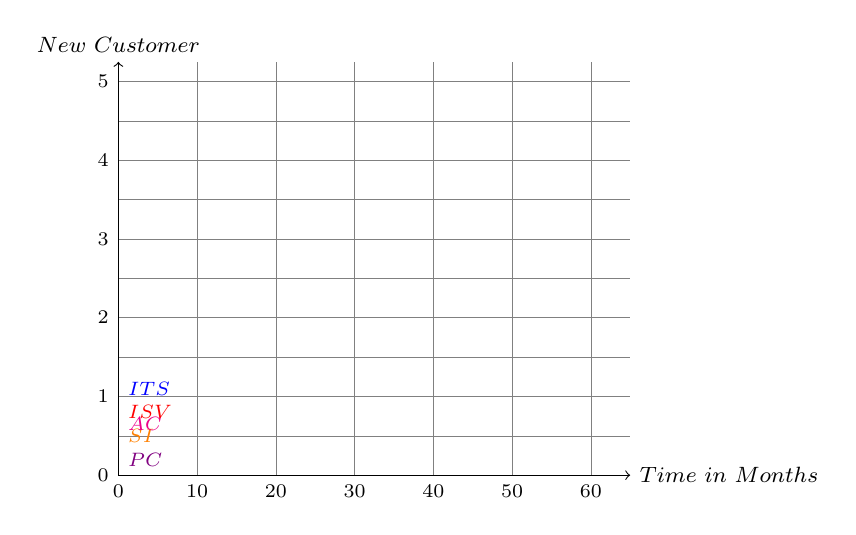
\begin{tikzpicture}[x=0.1cm,y=1cm]

  \def\xmin{0}
  \def\xmax{65}
  \def\ymin{0}
  \def\ymax{5.25}

  % grid
  \draw[style=help lines, ystep=0.5, xstep=10] (\xmin,\ymin) grid
  (\xmax,\ymax);

  % axes
  \draw[->] (\xmin,\ymin) -- (\xmax,\ymin) node[right] {\footnotesize $Time~in~Months$};
  \draw[->] (\xmin,\ymin) -- (\xmin,\ymax) node[above] {\footnotesize $New~Customer$};

  \foreach \x in {0,10,...,60}
    \node at (\x, \ymin) [below] {\scriptsize \x};
  \foreach \y in {0,1,...,5}
    \node at (\xmin,\y) [left] {\scriptsize \y};

  %,mark=*,mark size=0.5pt
	\draw[color=orange] plot[smooth] file {simulationData/SI/adoptionSI.txt}
			node [above=0.5cm, right] {\scriptsize $SI$};
	\draw[color=violet] plot[smooth] file {simulationData/PC/adoptionPC.txt}
			node [above=0.2cm, right] {\scriptsize $PC$};
	\draw[color=magenta] plot[smooth] file {simulationData/AC/adoptionAC.txt}
			node [above=0.65cm, right] {\scriptsize $AC$};
	\draw[color=red] plot[smooth] file {simulationData/ISV/adoptionISV.txt}
			node [above=0.8cm, right] {\scriptsize $ISV$};
	\draw[color=blue] plot[smooth] file {simulationData/ITS/adoptionITS.txt}
			node [above=1.1cm, right] {\scriptsize $ITS$};										
		
\end{tikzpicture}

	\caption{Proof of Concept -- Simulation Result}
	\label{fig:sim:ar}
\end{figure}

In the following the results of this simulation are discussed using the example of the adoption rates of all customer segments. A detailed overview is provided in Appendix \ref{ch:app05} by means of graphs for the most important overall modeling results as well as for each customer segment individually. Figure \ref{fig:sim:ar} illustrates the adoption rates of all customer segments. The sum of these adoption rates results in the variable new customers as calculated by Formula \ref{eq:nc}, which is illustrated in Figure \ref{fig:sim:nc}. Since the customer segment platform customers is served with the most sophisticated \ac{CVP}, its adoption rate reaches the peak first and hence the platform customer population increases quite fast and does so already at an early stage (cf. Figure \ref{fig:sim:pcs}). Somewhat surprisingly, the adoption rate of the customer segment \acp{SI} is second to reach its peak. The \ac{CVP} for \acp{SI} is rather low in comparison. However, this \ac{CVP} is influenced, among other things, by the platform customer market penetration which increases quite fast, based on the early and high adoption rate. Then, the adoption rate of the customer segment \acp{ISV} reaches its peak. This customer segments reaches the highest peak (representing the highest adoption rate in absolute terms), which can be explained by the proper \ac{CVP} and the early and high platform customer adoption rate, since the \ac{CVP} for \acp{ISV} is positively influenced by the market penetration of this customer segment. The adoption rate of the customer segment \ac{IT} startups reaches its peak next. Due to the fact that the \ac{CVP} for this customer segment is a little weaker compared to the \ac{ISV} \ac{CVP}, the \ac{IT} startup customer segment reaches the peak of its adoption rate later, and it is not as high as the customer segment \acp{ISV}. The lowest and latest adoption rate belongs to the customer segment application customers. The reasons for the shape of this adoption rate are the relatively low \ac{CVP} and the slow growth of the number of available platform modules (cf. Figure \ref{fig:sim:pm}). Since platform modules are developed by complementors, i.e. \acp{ISV} and \ac{IT} startups, these two customer segments need to growth first before the number of platform modules can increase with some delay. To sum up, the adoption simulation of the SAP HANA Cloud platform confirmed the previously revealed insights and made clear its weak points quantitatively. As well the fact that the number of platform modules currently available prevents the SAP HANA Cloud platform from establishing itself securely and from creating the crucial cross-sided network effects is revealed once again and brought into focus through the results of platform adoption simulation. Moreover, the simulation allows one to visualize both new and previously identified findings with the help of numbers and, more importantly, graphical presentations, thereby simplifying the communicability of these results and findings.

By applying the simulation model to the SAP HANA Cloud platform the example of a \ac{PoC} study is concluded. The application of the three \ac{DSR} artifacts to this platform has shown their applicability in the domain of \ac{PaaS} business models. First, using the classification scheme, \ac{PaaS} business models can be classified and, for instance, compared with other \ac{PaaS} business models. Thus initial insights concerning the business models currently pursued, e.g. weaknesses but also strengths, can be identified. Second, by utilizing the \acp{CLD} developed above these first insights can be investigated in more detail. Still, further insights may be revealed beyond this and will lead, in combination with the first insights, to a better understanding of the business model investigated. Third, by simulating the adoption of the examined \ac{PaaS} platform using the \ac{SFD} or simulation model, the insights gained so far can be quantified and further, as yet undiscovered insights may be found. All in all, the three \ac{DSR} artifacts, i.e. the classification scheme, \ac{CLD}, and \ac{SFD} or simulation model, facilitate a better understanding of the investigated \ac{PaaS} business model both in general and in particular with regard to the adoption dynamics.

\begin{comment}
	\begin{figure}[htb]
		\centering
		% ****************************************************************************************************
% Graph Population Customer Segments Stocks
% ****************************************************************************************************

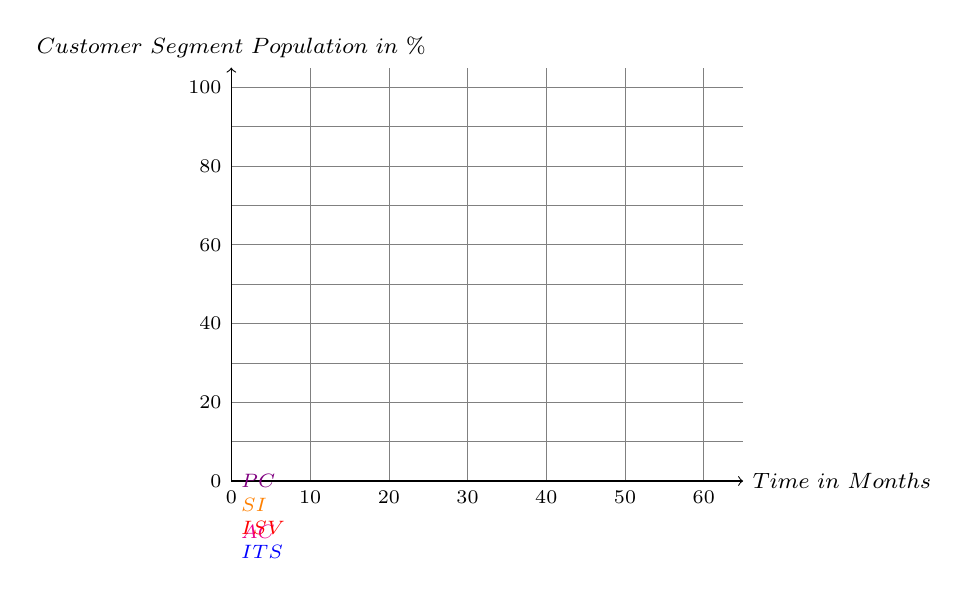
\begin{tikzpicture}[x=0.1cm,y=0.05cm]

  \def\xmin{0}
  \def\xmax{65}
  \def\ymin{0}
  \def\ymax{105}

  % grid
  \draw[style=help lines, ystep=10, xstep=10] (\xmin,\ymin) grid
  (\xmax,\ymax);

  % axes
  \draw[->] (\xmin,\ymin) -- (\xmax,\ymin) node[right] {\footnotesize $Time~in~Months$};
  \draw[->] (\xmin,\ymin) -- (\xmin,\ymax) node[above] {\footnotesize $Customer~Segment~Population~in~\%$};

  \foreach \x in {0,10,...,60}
    \node at (\x, \ymin) [below] {\scriptsize \x};
  \foreach \y in {0,20,...,100}
    \node at (\xmin,\y) [left] {\scriptsize \y};

  %,mark=*,mark size=0.5pt
	\draw[color=magenta] plot[smooth] file {simulationData/AC/populationAC.txt}
			node [below=0.65cm,right] {\scriptsize $AC$};
	\draw[color=blue] plot[smooth] file {simulationData/ITS/populationITS.txt}
			node [below=0.9cm,right] {\scriptsize $ITS$};	
	\draw[color=red] plot[smooth] file {simulationData/ISV/populationISV.txt}
			node [below=0.6cm,right] {\scriptsize $ISV$};	
	\draw[color=orange] plot[smooth] file {simulationData/SI/populationSI.txt}
			node [below=0.3cm,right] {\scriptsize $SI$};	
	\draw[color=violet] plot[smooth] file {simulationData/PC/populationPC.txt}
			node [right] {\scriptsize $PC$};	
												
\end{tikzpicture}

		\caption{Proof of Concept Simulation -- Customers}
	\end{figure}

	\begin{figure}[htb]
		\centering
		% ****************************************************************************************************
% Graph Potential Customer Segments Stocks
% ****************************************************************************************************

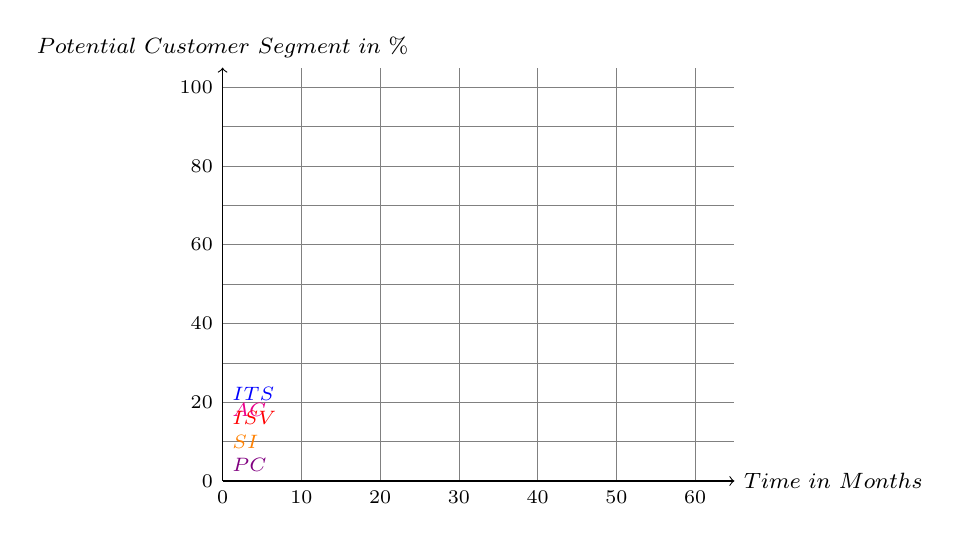
\begin{tikzpicture}[x=0.1cm,y=0.05cm]

  \def\xmin{0}
  \def\xmax{65}
  \def\ymin{0}
  \def\ymax{105}

  % grid
  \draw[style=help lines, ystep=10, xstep=10] (\xmin,\ymin) grid
  (\xmax,\ymax);

  % axes
  \draw[->] (\xmin,\ymin) -- (\xmax,\ymin) node[right] {\footnotesize $Time~in~Months$};
  \draw[->] (\xmin,\ymin) -- (\xmin,\ymax) node[above] {\footnotesize $Potential~Customer~Segment~in~\%$};

  \foreach \x in {0,10,...,60}
    \node at (\x, \ymin) [below] {\scriptsize \x};
  \foreach \y in {0,20,...,100}
    \node at (\xmin,\y) [left] {\scriptsize \y};

  %,mark=*,mark size=0.5pt
	\draw[color=magenta] plot[smooth] file {simulationData/AC/potentialAC.txt}
			node [above=0.9cm,right] {\scriptsize $AC$};
	\draw[color=blue] plot[smooth] file {simulationData/ITS/potentialITS.txt}
			node [above=1.1cm,right] {\scriptsize $ITS$};	
	\draw[color=red] plot[smooth] file {simulationData/ISV/potentialISV.txt}
			node [above=0.8cm,right] {\scriptsize $ISV$};	
	\draw[color=orange] plot[smooth] file {simulationData/SI/potentialSI.txt}
			node [above=0.5cm,right] {\scriptsize $SI$};	
	\draw[color=violet] plot[smooth] file {simulationData/PC/potentialPC.txt}
			node [above=0.2cm,right] {\scriptsize $PC$};	
	
													
\end{tikzpicture}

		\caption{Proof of Concept Simulation -- Potential Customers}
	\end{figure}
\end{comment}